\documentclass[14pt]{beamer} %Makes presentation

%\documentclass[handout]{beamer} %Makes Handouts
\usetheme{Singapore} %Gray with fade at top
\useoutertheme[subsection=false]{miniframes} %Supppress subsection in header
\useinnertheme{rectangles} %Itemize/Enumerate boxes
\usecolortheme{seagull} %Color theme
\usecolortheme{rose} %Inner color theme

\definecolor{light-gray}{gray}{0.75}
\definecolor{dark-gray}{gray}{0.55}
\setbeamercolor{item}{fg=light-gray}
\setbeamercolor{enumerate item}{fg=dark-gray}

\setbeamertemplate{navigation symbols}{}
%\setbeamertemplate{mini frames}[default]
%\setbeamercovered{dynamics}
\setbeamerfont*{title}{size=\Large,series=\bfseries}

%\setbeameroption{notes on second screen} %Dual-Screen Notes
%\setbeameroption{show only notes} %Notes Output

\setbeamertemplate{frametitle}{\vspace{.5em}\bfseries\insertframetitle}
\newcommand{\heading}[1]{\noindent \textbf{#1}\\ \vspace{1em}}

% small footnotes
\setbeamerfont{footnote}{size=\tiny}

\usepackage{bbding,color,multirow,times,ccaption,tabularx,graphicx,verbatim,booktabs,fixltx2e}
\usepackage{colortbl} %Table overlays
\usepackage[english]{babel}
\usepackage[latin1]{inputenc}
\usepackage[T1]{fontenc}
\usepackage{lmodern}
\usepackage{alltt}

\usepackage{tikz}
\usetikzlibrary{positioning}
\usetikzlibrary{trees}




\author[]{Thomas J. Leeper}
\institute[]{
  \inst{}%
  Department of Government\\London School of Economics and Political Science
}

\title{\large Some advice from a reproducible researcher about how some advice from research data repositories to irreproducible researchers about reproducibility and repositories might help researchers, repositories, and reproducibility}

\date[]{16 June 2017}

\begin{document}

\frame{\titlepage}

% advocates for reproducible research and those of you working with data repositories know why data archiving, curation, and reproducibility are important
% the median researcher does not know why these things are important and may very well not care
% reproducibility is just one more thing that researchers are asked to deal with, late in the research process, that isn't a publication and that doesn't lead to a publication

\frame{
    \frametitle{Why reproducibility?}
    \begin{itemize}\itemsep1em
        \item<1-> Journal requirements
        \item<1-> Funding agency requirements
        \item<1-> Institutional requirements
        \item<1-> The coming revolution
    \end{itemize}
    
    \vspace{1em}
    
    \onslide<2->{How can we shift thinking from \textit{extrinsic} motivations to intrinsic motivations?}
}

\frame{
    \frametitle{Getting intrinsic}

\begin{center}
    
\includegraphics[width=\textwidth]{images/nextweek}
\end{center}

}


\frame{
    \frametitle{What makes up the ideal reproducible research product?}
    
    \huge
    \onslide<2>{Nobody seems to agree!}
}

\frame{
    \begin{center}
        
\includegraphics[width=\textwidth]{images/badfolder}
    \end{center}
    
    \onslide<2->{Confession: This is my PhD dissertation.}
}

\frame<1>[label=ideal]{
    \frametitle{What makes up the ideal reproducible research product?}
    
   	\begin{itemize}\itemsep0.5em
   	\item Gandrud's template
   	\item rOpenSci's ``Research Compendium''
   	\item Project TIER
   	\item<2-> Docker container?
   	\item<3-> Virtual machine?
   	\item<4-> ???
   	\end{itemize}
    
    \onslide<5->{More is probably better for \textit{reproducibility}, but declining marginal returns for the researcher.}
    
}

\frame[label=gandrud]{
%%%%%%%%%%%%%%
% Example research project file path
% Christopher Gandrud
% Updated 21 October 2014
%%%%%%%%%%%%%%

% Set node styles
\tikzstyle{DirBox} = [draw=black,
                      rectangle,
                      minimum width=4em,
                      very thick,
                      font=\tiny]

\tikzstyle{every node} = [draw=gray,
                          thin,
                          anchor=west,
                          font=\tiny]

% Begin tikz picture
\begin{tikzpicture}[scale=0.9,%
  grow via three points={one child at (0.5,-0.7) and
  two children at (0.5,-0.7) and (0.5,-1.4)},
  edge from parent path={(\tikzparentnode.south) |- (\tikzchildnode.west)}]
  % Root Directory
  \node (root) at (5, 10) [DirBox]{Root};

  % Project Directory
  \node (project) at (4.425, 9) [DirBox]{Rep-Res-ExampleProject1}
        child {node {{\tiny{Paper.Rnw}}}}
        child {node {{\tiny{Slideshow.Rnw}}}}
        child {node {{\tiny{Website.Rnw}}}}
        child {node {{\tiny{Main.bib}}}}
            ;

  % Data Directory
  \node (data) at (0, 6.5) [DirBox]{Data}
      child {node {{\tiny{MainData.csv}}}}
      child {node {{\tiny{Makefile}}}}
      child {node {{\tiny{MergeData.R}}}}
      child {node {{\tiny{Gather1.R}}}}
      child {node {{\tiny{MainData\_VariableDescriptions.md}}}}
      child {node {{\tiny{README.Rmd}}}}
        ;

  % Analysis subdirectores/files
  \node (analysis) at (1.5, 8) [DirBox]{Analysis}
      child {node {{\tiny{GoogleVisMap.R}}}}
      child {node {{\tiny{ScatterUDSFert.R}}}}
        ;

  % README file
  \node (readme) at (9.5, 7) {README.md};

  % Connect boxes that are not explicit children
  \draw (root) -- (project);
  \draw (project) -| (analysis);
  \draw (analysis) -| (data);
  \draw (project) -| (readme);

\end{tikzpicture}
}


\begin{frame}[fragile, label=package]

\footnotesize

\begin{verbatim}
project
|- DESCRIPTION      # project metadata and dependencies 
|- README.md        # top-level description of content
|
|- data/            # raw data, not changed once created
|  +- my_data.csv   # data files in open formats
|
|- analysis/        # any programmatic code 
|  +- my_scripts.R  # R code used to analyse data 
\end{verbatim}

\end{frame}

\frame[label=tier]{
    \begin{center}
        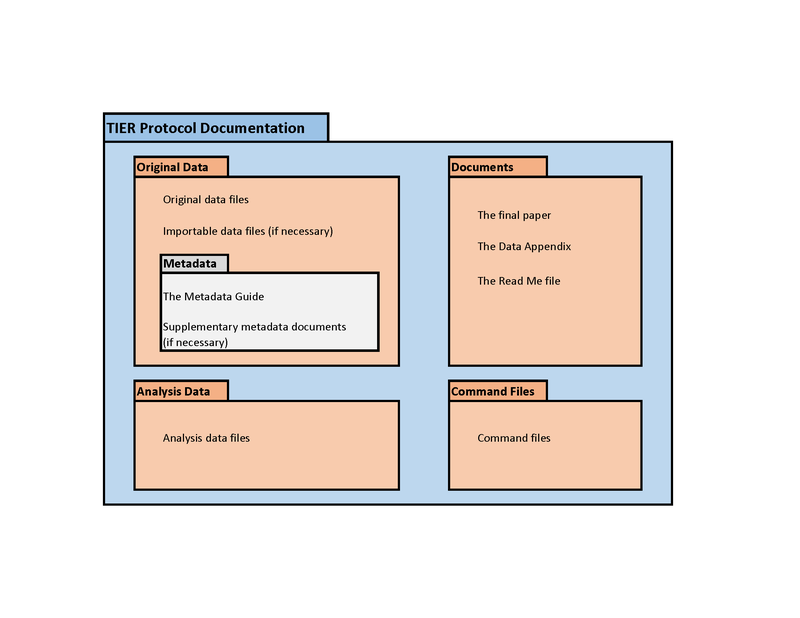
\includegraphics[width=\textwidth]{images/project-tier}
    \end{center}
}

\againframe{ideal}

\frame<1-2>[label=product]{
    \frametitle{What makes up the ideal reproducible research product?}
    
    \begin{itemize}\itemsep1em
    
    \item<1-> Big disagreements
    
    	\begin{itemize}\itemsep0.5em
    	\item What exactly is being reproduced?
    	\item What is being assumed about software, hardware, data formats, etc.?
    	\item What tools are best? packages? make? docker?
    	\end{itemize}
    
    \item<2-> Consensus is not possible! \onslide<3->{\textit{Nudge} instead.}
    
    	\begin{itemize}\itemsep0.5em
    	\item<4-> Provide templates to use when \textit{starting} a project
    	\item<5-> Provide varied exemplars to show how to conceptualize the organization of a project
    	\end{itemize}
    
    \end{itemize}
}

\frame{
    \begin{center}
        
\includegraphics[width=\textwidth]{images/xkcd927}
    \end{center}
}

\againframe<2->{product}


\frame{
    \begin{center}
        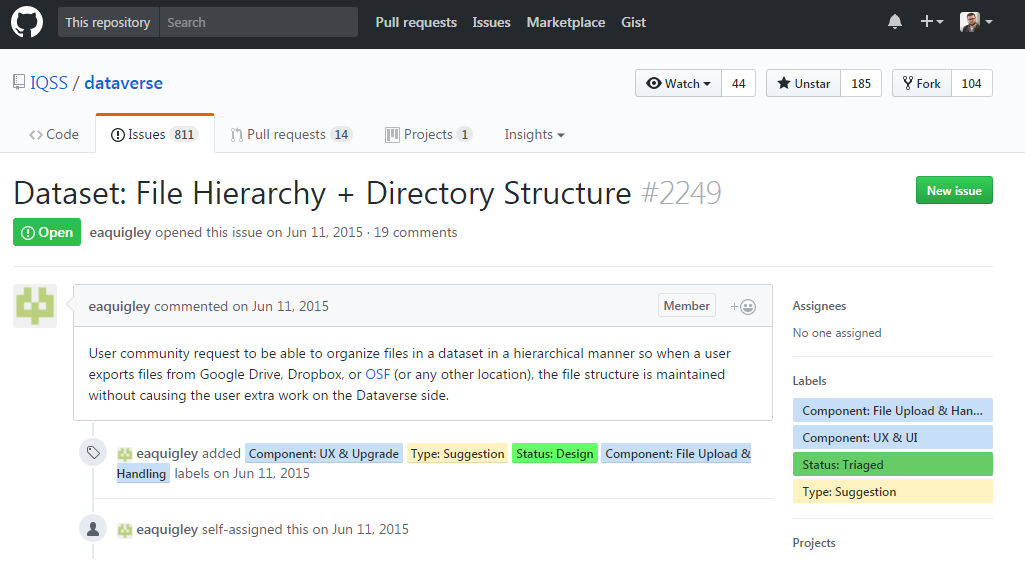
\includegraphics[width=\textwidth]{images/issue2249}
    \end{center}
}

\frame{
    \begin{center}
        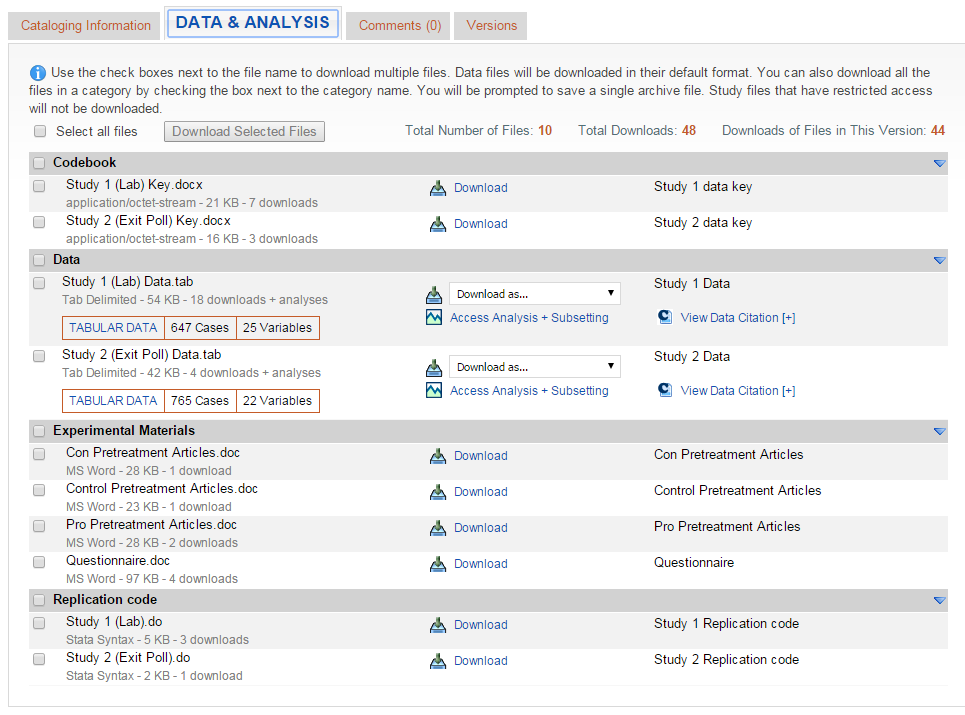
\includegraphics[width=\textwidth]{images/dataverseorganized}
    \end{center}
}

\frame{
    \begin{center}
        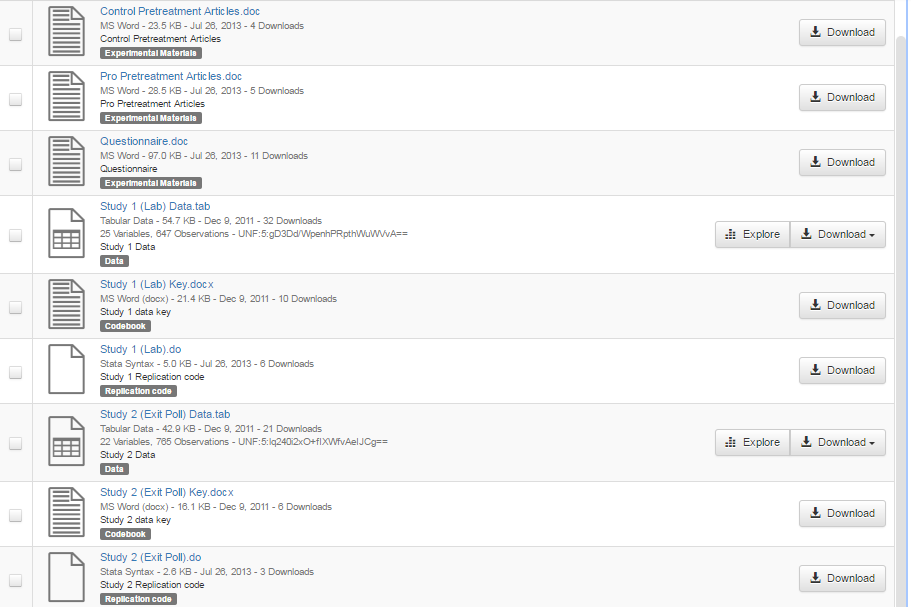
\includegraphics[width=\textwidth]{images/dataverse4}
    \end{center}
}



\frame{
    \frametitle{The Advice to Researchers}
    
    \begin{enumerate}\itemsep1em
        \item Reproducibility isn't just one more burden
        \item It's about helping your (future) \textit{yourself} first
        \item Be reproducible for science second
    \end{enumerate}
    
    \vspace{1em}
    
    \onslide<2->{}
}

\frame{
	\begin{center}
		
\includegraphics[height=.9\textheight]{images/xkcd1421}
	\end{center}
}


% Repositories need to help researchers \textit{start} their project reproducibly. That means helping them get organized, early.


\bgroup
\setbeamercolor{background canvas}{bg=black}
\setbeamertemplate{navigation symbols}{}
\begin{frame}[plain]{}
\end{frame}
\egroup


\appendix
\frame{}


\frame{
    \frametitle{\textit{Ir}reproducibility}
    \begin{itemize}\itemsep0.25em
        \item<2-> Fabrication
        \item<3-> Human error
        \item<4-> Lack of methodological transparency
        \item<5-> Proprietary data and file formats
        \item<6-> Unavailable data
        \item<7-> Analysis uses proprietary software/hardware
        \item<8-> Analysis unavailable
        \item<9-> ``Available from the author\only<11->{ (now deceased)}'' 
    \end{itemize}
}

\frame{
\begin{center}
    
\includegraphics[width=\textwidth]{images/bullshit}
\end{center}
}


\end{document}
